\documentclass[11pt,a4paper]{article}

\usepackage[margin=1in]{geometry}
\usepackage{amsmath,amssymb,amsthm}
\usepackage{booktabs}
\usepackage{array}
\usepackage{listings}
\usepackage{xcolor}
\usepackage[expansion=false]{microtype}
\usepackage{enumitem}
\usepackage{tikz}
\usepackage{float}
\usepackage[hidelinks]{hyperref}

\usetikzlibrary{arrows,decorations.pathmorphing,calc}
\tikzset{>=stealth'}

\definecolor{codebg}{HTML}{F5F5F5}
\definecolor{ribL}{HTML}{7F77DD}
\definecolor{ribR}{HTML}{1D9E75}
\definecolor{amb}{HTML}{EF9F27}

\lstset{
  basicstyle=\ttfamily\footnotesize,
  backgroundcolor=\color{codebg},
  frame=single, framesep=4pt, rulecolor=\color{black!20},
  breaklines=true, columns=fullflexible, keepspaces=true,
  showstringspaces=false, xleftmargin=0pt, aboveskip=1em, belowskip=1em
}

\newcommand{\MUST}{\textsc{must}}
\newcommand{\MUSTNOT}{\textsc{must not}}
\newcommand{\SHOULD}{\textsc{should}}
\newcommand{\SHOULDNOT}{\textsc{should not}}
\newcommand{\MAY}{\textsc{may}}

\theoremstyle{definition}
\newtheorem{definition}{Definition}
\theoremstyle{plain}
\newtheorem{proposition}{Proposition}
\theoremstyle{remark}
\newtheorem*{decision}{Decision required}

% ---------------------------------------------------------------- scene macros
\newcommand{\spools}{%
  \fill[ribL,opacity=.45,rounded corners=2pt] (1.55,5.40) rectangle (2.45,5.95);
  \fill[ribR,opacity=.45,rounded corners=2pt] (5.55,5.40) rectangle (6.45,5.95);
  \node[font=\scriptsize] at (2,6.22) {left spool};
  \node[font=\scriptsize] at (6,6.22) {right spool};
}
\newcommand{\musician}{%
  \draw[gray] (4,-0.10) circle (0.23);
  \node[font=\scriptsize] at (4,-0.10) {M};
}
\newcommand{\axes}{%
  \draw[->,gray,thin] (0.85,4.30) -- (1.45,4.30) node[right,font=\scriptsize]{$x$};
  \draw[->,gray,thin] (0.85,4.30) -- (0.85,4.90) node[above,font=\scriptsize]{$z$};
}
\newcommand{\ribbonsopen}{%
  \draw[ribL,opacity=.45,line width=16pt,line join=round]
    (2,5.40) -- (2,4.60) -- (3.10,4.00) -- (3.10,0.70);
  \draw[ribR,opacity=.45,line width=16pt,line join=round]
    (6,5.40) -- (6,4.60) -- (4.90,4.00) -- (4.90,0.70);
}
\newcommand{\ribbonszipped}{%
  \draw[ribL,opacity=.45,line width=16pt,line join=round]
    (2,5.40) -- (2,4.60) -- (3.72,4.20) -- (3.72,2.20) -- (3.10,1.70) -- (3.10,0.70);
  \draw[ribR,opacity=.45,line width=16pt,line join=round]
    (6,5.40) -- (6,4.60) -- (4.28,4.20) -- (4.28,2.20) -- (4.90,1.70) -- (4.90,0.70);
}
\newcommand{\mesh}[2]{%
  \draw[gray!75,decorate,decoration={zigzag,segment length=5pt,amplitude=3pt}]
    (4,#1) -- (4,#2);
}
\newcommand{\mountclips}{%
  \fill[amb,opacity=.75,rounded corners=1pt] (3.76,1.05) rectangle (3.92,1.45);
  \fill[amb,opacity=.75,rounded corners=1pt] (4.08,1.05) rectangle (4.24,1.45);
}
\newcommand{\handat}[2]{\filldraw[fill=white,draw=gray!80,thin] (#1,#2) circle (0.17);}
\newcommand{\handsdefault}{\handat{3.10}{0.55}\handat{4.90}{0.55}}

\title{\textbf{The F1R3Skein Virtual Instrument}\\[0.3em]
\large Specification, revision 3}
\author{F1R3FLY.io}
\date{4 September 2026}

\begin{document}
\maketitle

\begin{abstract}
\noindent
This document specifies the F1R3Skein virtual instrument: the gestural surface through which a
musician draws melody out of the digit streams of mathematical constants, and out of which the
platform's two primary artifacts---tunes and performances---are produced.

Revision 3 replaces the instrument's physical model rather than adjusting it. The two streams now
have separate spools, separately mobile, spread apart on the $x$-axis. Ribbon spools toward the
musician and divides into future, present and past. The ribbons carry notches on their inner
edges; bringing them together meshes those notches, and the mesh propagates as a wave into the
future. A notch pair is a note, the zip front is the playhead, and the wave's speed is the tempo.
Capture is a two-handed act performed against a mount that takes over the holding.

The gesture vocabulary grows from six to nine, each specified here with a diagram. Three
consequences are structural and are flagged where they arise: the recogniser needs a trajectory
detector as well as pose tests, it needs modes, and the cut carries two positions rather than none.
Section~\ref{sec:decisions} lists what remains open.
\end{abstract}

\tableofcontents

\section{Scope and conformance}

In scope: the generative core, the playing surface and its geometry, the instrument's state model,
the gesture vocabulary and its detection criteria, the wire protocol, the visual and audio models,
performance recording, and the budgets that make the instrument playable.

Out of scope: identity, galleries, the engagement ledger, breeding and selection, and the on-chain
representation of tunes. This document defines what the instrument \emph{produces}.

\MUST, \MUSTNOT, \SHOULD, \SHOULDNOT{} and \MAY{} are used in the sense of RFC 2119.
\emph{M} denotes the musician throughout.

\subsection{Terminology}

\begin{description}[leftmargin=2.4cm,style=nextline,font=\normalfont\itshape]
\item[Engine] The process holding authoritative instrument state.
\item[Client] The visionOS application: gesture recognition, rendering, audio.
\item[Stream] One spigot: a constant, an output base, a cursor position.
\item[Spool] The visible source of one stream, far from M on the $z$-axis.
\item[Ribbon] The visible material spooling from one spool toward M.
\item[Notch] One digit position, presented on a ribbon's inner edge.
\item[Skein] The pair of ribbons together with their relative registration.
\item[Zip front] The boundary where unmeshed ribbon becomes meshed. The playhead.
\item[Tune] A snipped, named artifact.
\item[Performance] The recorded trace of a session.
\end{description}

\section{Deployment configurations}

\begin{description}[leftmargin=1cm,style=nextline]
\item[\textbf{S1 --- Tethered.}] Engine on a Mac, client on the headset, TCP over the local network
with Bonjour discovery. September test configuration; explicitly a stopgap.
\item[\textbf{S2 --- On-device.}] Engine built for \texttt{arm64-apple-visionos} as a
static library behind a C foreign-function interface. No transport at all. The target.
\end{description}

The protocol of Section~\ref{sec:protocol} is defined over an abstract bidirectional channel; in S1
that is a TCP stream, in S2 a pair of FFI ring buffers. No other part of this specification
distinguishes them, and the client \MUSTNOT{} contain transport-specific logic outside its channel
implementation.

The Unix-domain-socket transport \MUSTNOT{} be used for device testing: a Unix socket is addressed
by a path in one host's filesystem, and the headset is a different host.

\section{The generative core}

\subsection{Streams}

The engine \MUST{} provide the five constants---$\pi$, $e$, $\varphi$, $\ln 2$, Liouville's---each
emitting digits in a configurable base $b$, $2 \le b \le 36$. Emission \MUST{} be exact and
unbounded. A stream configuration is a pair $(c,b)$; with a cursor position $p$ it determines the
digit $d(c,b,p)$ uniquely.

The $\pi$ implementation \SHOULD{} move to Bailey--Borwein--Plouffe extraction where the base
permits, and \MUST{} memoise emitted digits so re-realisation of a visited range is $O(1)$ per
digit. Deep positions are exactly what a long session produces.

\subsection{Two cursors, separately mobile}

The skein holds two configurations and two \emph{independent} cursor positions, $p_L$ and $p_R$.
Independence is the point of the design and \MUST{} be preserved: it is what lets M hold a rhythmic
motif fixed while advancing pitch, or dually.

\begin{proposition}[The instrument performs its own algebra]
Holding one ribbon fixed and meshing a different segment of the other against it takes the
durations of one candidate and the pitches of another. That is the crossover operator
$\mathsf{XPitch}$ of the breeding engine, performed by hand; its dual is
$\mathsf{XPitch}(f,m)$ by the rectangular-band identity. Selection and reproduction are not a
subsystem bolted onto a music toy---the population does at scale what M does at the bench.
\end{proposition}

\subsection{Note mapping}

One stream governs pitch, the other duration; \emph{twist} exchanges the roles. For the $k$-th
meshed notch pair the engine \MUST{} produce
$(\Pi(d_{\text{pitch}}),\ \Delta(d_{\text{duration}}))$. Both maps \MUST{} be session parameters,
not build constants. Pitch maps \MUST{} include major, minor, pentatonic major, pentatonic minor,
Dorian, whole tone and chromatic over a configurable root; duration maps \MUST{} include musical,
linear, exponential and fixed. A stream's base \SHOULD{} match the cardinality of the map it drives.

\section{The playing surface}
\label{sec:surface}

Axes are M's: $x$ is left--right, $y$ is up--down, $z$ is depth away from M.

Each stream has its own spool. The two spools sit at the \emph{same height} and are spread apart on
the $x$-axis, far from M on $z$. Ribbon spools from each toward M's hands. Each ribbon divides into
three sections:

\begin{description}[leftmargin=1.6cm,style=nextline]
\item[\textbf{Future}] still wound on the spool, unseen.
\item[\textbf{Present}] between the spool and M's hands, visible.
\item[\textbf{Past}] having passed the hands, hanging below them toward the floor.
\end{description}

Each ribbon carries notches on its \emph{inner} edge---the edge facing the other ribbon. Bringing
the ribbons together meshes the notches over a section of the present, leaving unmeshed margins
near the hands and near the spools. The mount sits between the ribbons, just in front of the hands,
and is a pair of clips.

\begin{figure}[H]\centering
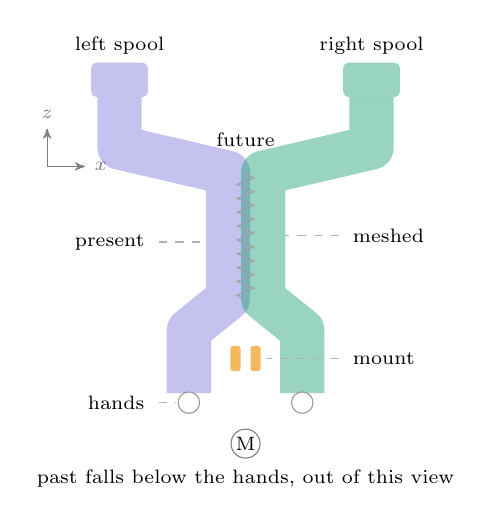
\begin{tikzpicture}[scale=0.80]
\axes \spools \ribbonszipped \mesh{2.20}{4.20} \mountclips \handsdefault \musician
\node[font=\scriptsize] at (4,4.72) {future};
\node[font=\scriptsize,anchor=east] at (2.55,3.10) {present};
\draw[gray!60,thin,dashed] (2.62,3.10) -- (3.38,3.10);
\node[font=\scriptsize,anchor=west] at (5.55,3.20) {meshed};
\draw[gray!60,thin,dashed] (5.48,3.20) -- (4.62,3.20);
\node[font=\scriptsize,anchor=west] at (5.55,1.25) {mount};
\draw[gray!60,thin,dashed] (5.48,1.25) -- (4.32,1.25);
\node[font=\scriptsize,anchor=east] at (2.55,0.55) {hands};
\draw[gray!60,thin,dashed] (2.62,0.55) -- (2.90,0.55);
\node[font=\scriptsize] at (4,-0.65) {past falls below the hands, out of this view};
\end{tikzpicture}
\caption{The playing surface, seen from above. Two spools at the same height, spread on $x$.}
\end{figure}

\begin{quote}
\textbf{A notch pair is a note.} Meshing commits notch $k$ on the left to notch $k$ on the right.
While unmeshed the ribbons slide independently and M sets the relative phase; once meshed the
pairing is fixed. Independent mobility and well-formed pairing are not in tension---they are
separated in time by the zip.
\end{quote}

\section{Instrument state}

\[
\Sigma = \big\langle\;
(c_L,b_L,p_L),\; (c_R,b_R,p_R),\;
\zeta,\; \mu,\; \lambda,\;
\Pi,\Delta,\tau,\iota,\; T
\;\big\rangle
\]

with $\zeta$ the zip state (unzipped, or zipped with a front position and a propagation rate),
$\mu$ the mount state, $\lambda$ the loop state, $\tau$ tempo, $\iota$ instrument, $T$ the tune
tray. The client \MUSTNOT{} hold authoritative state; it renders $\Sigma$ and emits gestures.

\section{Gesture vocabulary}
\label{sec:gestures}

Nine gestures. Each subsection gives the physical form, the effect, and a diagram of the surface
during that gesture.

\subsection{Pull}

M draws one hand toward herself, advancing that stream. Step count is proportional to speed. Pulls
are per-hand and independent; this is where the relative phase between the two streams is set.

\begin{figure}[H]\centering
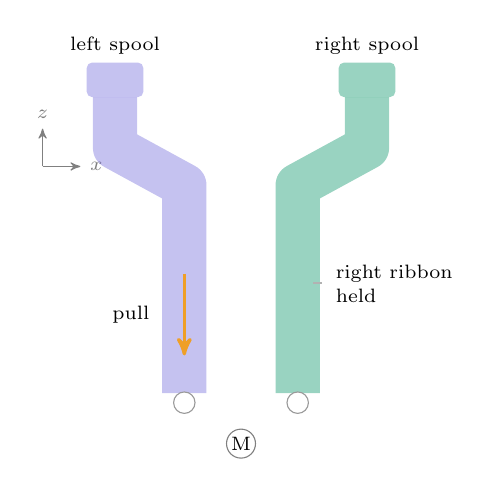
\begin{tikzpicture}[scale=0.80]
\axes \spools \ribbonsopen \handsdefault \musician
\draw[->,amb,very thick] (3.10,2.60) -- (3.10,1.30);
\node[font=\scriptsize,anchor=east] at (2.70,1.95) {pull};
\node[font=\scriptsize,anchor=west] at (5.35,2.60) {right ribbon};
\node[font=\scriptsize,anchor=west] at (5.35,2.25) {held};
\draw[gray!60,thin,dashed] (5.28,2.45) -- (5.12,2.45);
\end{tikzpicture}
\caption{Pull. Ribbons unmeshed; each advances alone. Holding one and pulling the other is how M
chooses which rhythm meets which pitches.}
\end{figure}

\subsection{Twist}

One hand held clearly above the other, hands apart. Exchanges the two streams, cursors included.
Twist \MUST{} be permitted only while unzipped: the mesh commits the pairing, and exchanging roles
underneath a committed mesh has no coherent reading.

\begin{figure}[H]\centering
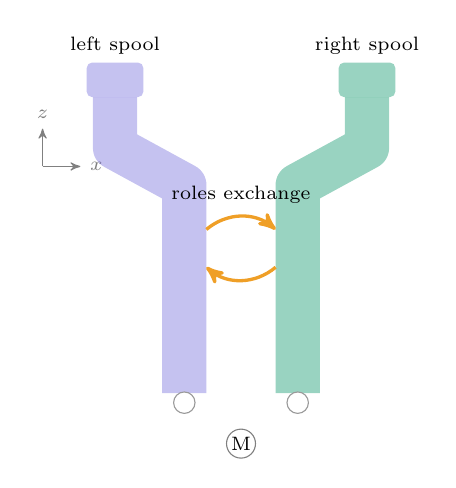
\begin{tikzpicture}[scale=0.80]
\axes \spools \ribbonsopen \handsdefault \musician
\draw[->,amb,very thick] (3.45,3.30) to[out=40,in=140] (4.55,3.30);
\draw[->,amb,very thick] (4.55,2.70) to[out=220,in=320] (3.45,2.70);
\node[font=\scriptsize] at (4,3.85) {roles exchange};
\end{tikzpicture}
\caption{Twist. Which stream governs pitch and which governs duration is swapped. Permitted only
while unzipped.}
\end{figure}

\subsection{Zip}

M brings the two ribbons together. The notches mesh, and \textbf{the mesh keeps going}: the zip
front propagates away from M into the future without further input. As the meshed section outgrows
the present, the spools appear to recede to supply more ribbon.

The zip front is the playhead. Each notch pair sounds as it engages, so zipping \emph{is} playing,
and the propagation rate is the tempo.

\begin{figure}[H]\centering
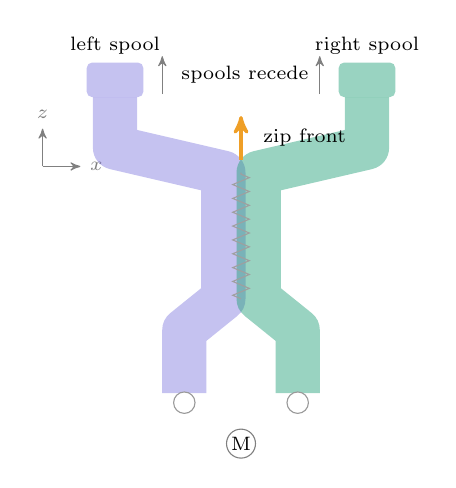
\begin{tikzpicture}[scale=0.80]
\axes \spools \ribbonszipped \mesh{2.20}{4.20} \handsdefault \musician
\draw[->,amb,very thick] (4,4.40) -- (4,5.10);
\node[font=\scriptsize,anchor=west] at (4.20,4.75) {zip front};
\draw[->,gray,thin] (2.75,5.45) -- (2.75,6.05);
\draw[->,gray,thin] (5.25,5.45) -- (5.25,6.05);
\node[font=\scriptsize,anchor=west] at (2.90,5.75) {spools recede};
\end{tikzpicture}
\caption{Zip. The wave propagates into the future unaided; the spools retreat to feed it. Each
notch pair sounds as it engages.}
\end{figure}

\subsection{Halt --- stopping the wave}
\label{sec:halt}

M looks at the zip front and stops it. The wave freezes, the spools stop receding, and a short
unmeshed reserve remains between the meshed section and the spools.

\begin{quote}
\textbf{Platform constraint.} visionOS does not expose gaze to applications. Hover highlighting is
rendered out-of-process by the system and is not reported to the app, and there is no
\texttt{onHover} equivalent: the application learns nothing until the user commits. A continuous
``M looks and the wave halts'' therefore cannot be built.
\end{quote}

\begin{sloppypar}
The realisable form preserves the intent. The zip front entity \MUST{} carry a
\texttt{HoverEffectComponent}, so the system highlights it as M looks---costing us nothing and
leaking nothing---and M commits with a small pinch, which reaches the app as a spatial tap
carrying its 3D location. Her eyes still aim; the pinch is only the trigger, and the zip front
is the one thing out there to look at.
\end{sloppypar}

Head direction \MUSTNOT{} be substituted as a gaze proxy. A musician's head moves constantly and
independently of her eyes; the wave would halt every time she glanced at the tray.

\begin{figure}[H]\centering
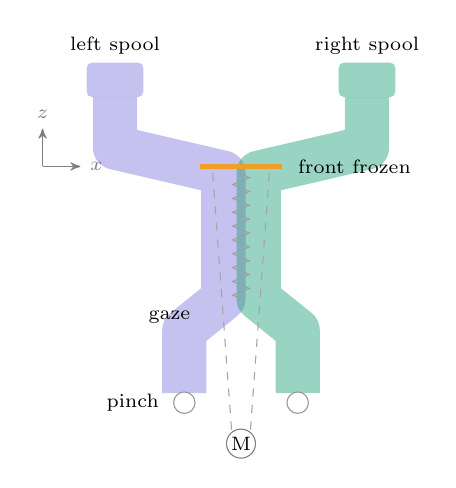
\begin{tikzpicture}[scale=0.80]
\axes \spools \ribbonszipped \mesh{2.20}{4.20} \handsdefault \musician
\draw[amb,line width=2pt] (3.35,4.30) -- (4.65,4.30);
\draw[gray!70,thin,dashed] (3.85,0.12) -- (3.55,4.20);
\draw[gray!70,thin,dashed] (4.15,0.12) -- (4.45,4.20);
\node[font=\scriptsize,anchor=west] at (4.75,4.30) {front frozen};
\node[font=\scriptsize,anchor=east] at (2.85,0.55) {pinch};
\node[font=\scriptsize,anchor=east] at (3.35,1.90) {gaze};
\end{tikzpicture}
\caption{Halt. M looks at the front; the system highlights it; a pinch commits. The unmeshed
reserve above the front is what a later zip resumes from.}
\end{figure}

\subsection{Unzip}

Separates the ribbons, retiring the mesh from the near end. Unzipping is what lets M re-set the
relative phase and mesh a different segment against a held ribbon---the crossover move of
Proposition~1.

\begin{figure}[H]\centering
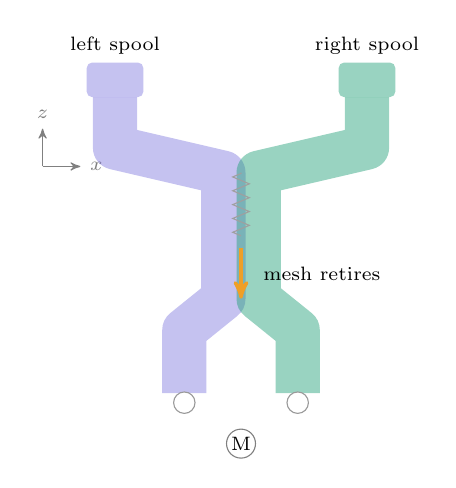
\begin{tikzpicture}[scale=0.80]
\axes \spools \ribbonszipped \mesh{3.20}{4.20} \handsdefault \musician
\draw[->,amb,very thick] (4,3.00) -- (4,2.20);
\node[font=\scriptsize,anchor=west] at (4.20,2.60) {mesh retires};
\end{tikzpicture}
\caption{Unzip. The pairing is released from the near end, freeing the ribbons to slide
independently again.}
\end{figure}

\subsection{Mount}

M slots the unmeshed lead of each ribbon into the clips. \textbf{The mount's job is to take over the
holding.} Until this moment each hand has been driving its own ribbon; once clipped, both hands are
free to leave their stations and travel out along the meshed band without the assembly collapsing
into the past. This is why mounting \MUST{} precede snipping.

The mount contributes no boundary to the captured tune.

\begin{figure}[H]\centering
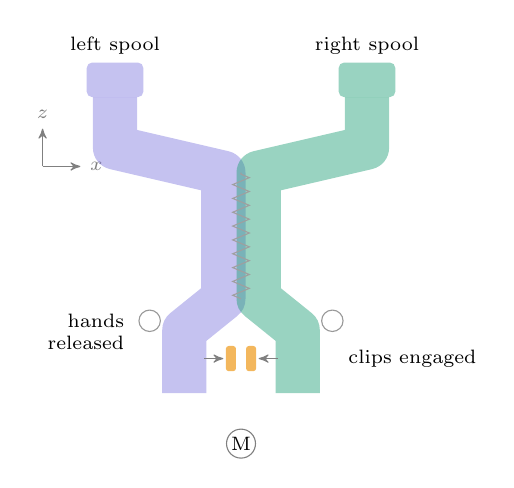
\begin{tikzpicture}[scale=0.80]
\axes \spools \ribbonszipped \mesh{2.20}{4.20} \mountclips \musician
\handat{2.55}{1.85}\handat{5.45}{1.85}
\draw[->,gray,thin] (3.42,1.25) -- (3.72,1.25);
\draw[->,gray,thin] (4.58,1.25) -- (4.28,1.25);
\node[font=\scriptsize,anchor=west] at (5.55,1.25) {clips engaged};
\node[font=\scriptsize,anchor=east] at (2.30,1.85) {hands};
\node[font=\scriptsize,anchor=east] at (2.30,1.50) {released};
\end{tikzpicture}
\caption{Mount. Two clips take the load; M's hands are freed for the two-handed snip.}
\end{figure}

\subsection{Loop}

A circular finger motion---the ``go on'' gesture---sets the meshed section looping so M can audition
it. The loop span runs from the mount to the halted zip front. Reversing the direction of rotation
clears the loop.

Looping needs no new machinery in the representation: repetition is $\mathsf{Seq}$ of copies, which
the monoid already supplies. Loop is a transport control, recorded in the performance trace, and
leaves the tune term untouched.

\begin{figure}[H]\centering
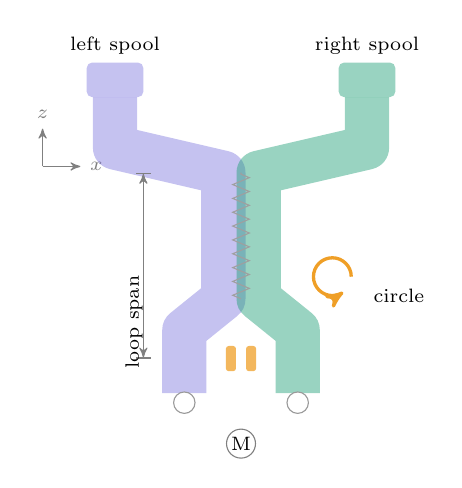
\begin{tikzpicture}[scale=0.80]
\axes \spools \ribbonszipped \mesh{2.20}{4.20} \mountclips \handsdefault \musician
\draw[->,amb,very thick] (5.75,2.55) arc (0:305:0.30);
\node[font=\scriptsize,anchor=west] at (5.95,2.25) {circle};
\draw[|<->|,gray] (2.45,1.25) -- (2.45,4.20);
\node[font=\scriptsize,anchor=east,rotate=90] at (2.30,2.72) {loop span};
\end{tikzpicture}
\caption{Loop. Mount to halted front. Audition wide, cut narrow.}
\end{figure}

\subsection{Snip}

\textbf{Both hands are involved.} One hand is nearest M, the other nearest the spools; what is
snipped is the section \emph{between the hands}. Two cut planes free a middle piece that is already
gripped at both ends, so M carries it to the tray rather than watching it drop---which is the
physical reason a snip needs two hands.

\begin{itemize}[leftmargin=*]
\item The near hand supplies $i_L$ and $i_R$; the separation of the hands in notches supplies $n$.
\item Roles are assigned by $z$-ordering at the moment of the gesture, \MUSTNOT{} by chirality.
      Either hand may be the near one.
\item Both cuts \MUST{} land inside the meshed span. Cutting the unmeshed lead would free two loose
      ribbons rather than a tune.
\item The cut \MUST{} be previewed: while the pose is held, a marker tracks each hand along the
      band so M can slide to the right notch before closing.
\end{itemize}

M is free to cut a smaller section than the full extent from mount to front---that is her choice,
and it is why the three decisions are independent: the mount fixes where holding is taken over,
halting fixes how much material exists, the cut fixes how much she keeps.

\begin{figure}[H]\centering
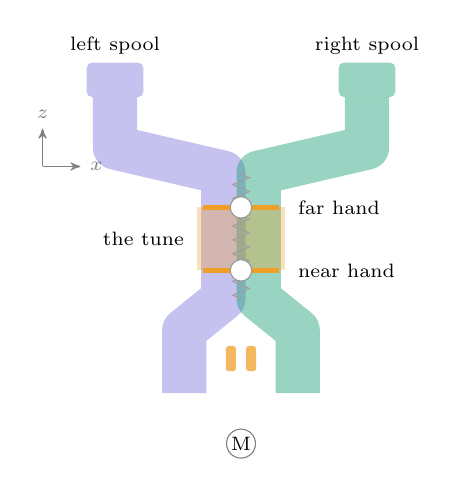
\begin{tikzpicture}[scale=0.80]
\axes \spools \ribbonszipped
\draw[amb,opacity=.32,line width=32pt] (4,2.65) -- (4,3.65);
\mesh{2.20}{4.20} \mountclips \musician
\draw[amb,line width=1.6pt] (3.40,2.65) -- (4.60,2.65);
\draw[amb,line width=1.6pt] (3.40,3.65) -- (4.60,3.65);
\handat{4.00}{2.65}\handat{4.00}{3.65}
\node[font=\scriptsize,anchor=west] at (4.75,2.65) {near hand};
\node[font=\scriptsize,anchor=west] at (4.75,3.65) {far hand};
\node[font=\scriptsize,anchor=east] at (3.25,3.15) {the tune};
\end{tikzpicture}
\caption{Snip. Two cuts, both inside the mesh. What is between the hands becomes the tune; the
piece is held at both ends as it is freed.}
\end{figure}

\subsection{Modes and mutual exclusion}

Three rules are new in this revision and one of them is not optional.

\paragraph{Cut mode is mandatory.} Moving a hand along $z$ \emph{is} the pull gesture. During a
snip M does exactly that with both hands, travelling out along the band to bracket a section. Pull
therefore \MUST{} be suppressed between mounting and the completion or abandonment of a snip.
Without this the streams advance while M is choosing a cut. The current recogniser has no notion of
mode---every predicate is evaluated every frame against every hand---so this is more invasive than
adding a gesture, and it produces baffling behaviour if discovered late.

\paragraph{Circling must not read as pulling.} A circling hand crosses the pull velocity threshold
twice per revolution. Loop and pull \MUST{} be mutually excluded.

\paragraph{Twist requires unzipped.} As \S6.2.

The rules retained from revision 2: gestures are edge-triggered with cooldowns and \MUSTNOT{}
re-fire while a pose is held; zip and twist are never simultaneously satisfiable.

\subsection{Two kinds of detector}

Every gesture in the current recogniser is a per-frame pose test plus a frame counter. The loop
gesture is a \emph{trajectory}, and the recogniser \MUST{} therefore grow a second kind of
detector: a ring buffer of index-fingertip positions, a plane fit over the window, the unwrapped
angle accumulated about the centroid, firing when the sweep passes $2\pi$ with radius variance and
plane residual inside bounds. Direction of rotation comes free and gives loop-set against
loop-clear.

\subsection{Detection parameters}

Every threshold \MUST{} live in an external calibration profile, loaded at launch and reloadable
without a rebuild. Hardcoded constants \MUSTNOT{} remain in the recogniser.

\begin{center}
\begin{tabular}{lll}
\toprule
\textbf{Parameter} & \textbf{Governs} & \textbf{Provisional} \\
\midrule
\texttt{pull.velocity\_min}    & speed toward M            & 0.25 m/s \\
\texttt{pull.step\_divisor}    & speed to step count       & 0.15 \\
\texttt{pull.cooldown}         & minimum interval          & 0.08 s \\
\texttt{zip.distance}          & ribbons-together          & 0.10 m \\
\texttt{unzip.distance}        & ribbons-apart             & 0.22 m \\
\texttt{twist.height\_delta}   & vertical offset           & 0.06 m \\
\texttt{twist.hold\_frames}    & frames before firing      & 8 \\
\texttt{scissors.spread}       & index/middle angle        & 0.40 rad \\
\texttt{scissors.extended}     & extension floor           & \emph{to be derived} \\
\texttt{scissors.curled}       & curl ceiling              & \emph{to be derived} \\
\texttt{loop.min\_radius}      & circle size floor         & \emph{to be derived} \\
\texttt{loop.radius\_variance} & circularity tolerance     & \emph{to be derived} \\
\texttt{loop.plane\_residual}  & planarity tolerance       & \emph{to be derived} \\
\bottomrule
\end{tabular}
\end{center}

\subsection{Finger curl must be scale-invariant}

The implemented curl metric is $\lVert\text{tip}-\text{metacarpal}\rVert/0.08$ clamped to unity,
with ``curled'' asserted below $0.30$. A fully curled adult ring finger measures roughly
$0.06$--$0.08$\,m tip-to-metacarpal, giving $0.75$--$1.0$. The threshold is unreachable and scissors
never fires. The metric is also not scale-invariant: the fixed divisor makes detection depend on
hand size.

Curl \MUST{} instead be the interior angle at the proximal interphalangeal joint, or tip-to-wrist
distance normalised by that finger's own summed segment lengths. Thresholds \MUST{} be derived from
recorded traces (\S\ref{sec:instrumentation}), not chosen by inspection.

\section{Snip semantics and the tune term}
\label{sec:snip}

\subsection{The defect being corrected}

The engine currently derives a snip from the \emph{left} cursor alone: it computes
$\textit{from}=p_L-w$ and $\textit{to}=p_L$ for ribbon width $w$, then advances both fresh spigots
to \textit{from}. Since $p_L$ and $p_R$ are independent by design, the stored snippet is
$(d(c_L,b_L,k), d(c_R,b_R,k))_{k}$ over a single index, while what M heard was
$(d(c_L,b_L,i), d(c_R,b_R,j))$ with $i$ and $j$ independent.

\begin{quote}\itshape
A snipped tune is, in general, not the tune M heard.
\end{quote}

A third representation compounds it: the tray receives the digits actually displayed, while the
snippet map receives the re-derived pairs. ``The snipped tune'' denotes three different things
depending on where one looks.

\subsection{Resolution}

\[
\mathsf{Snip}(k,\; i_L,\; i_R,\; n)
\quad\text{denoting}\quad
\big(d(c_L,b_L,i_L+t),\ d(c_R,b_R,i_R+t)\big)_{t\in[0,n)} .
\]

The mesh guarantees equal counts on both sides, so a common length $n$ is exact rather than
assumed. The near hand supplies $i_L$ and $i_R$; the hand separation supplies $n$. Tray, snippet map
and realised audio \MUST{} all derive from this one term.

\subsection{Consequences}

\paragraph{The Theory of skeins.} \texttt{Skein.module} currently declares
\begin{lstlisting}
Snip . k:Skein, i:Nat, j:Nat |- "snip" "(" k "," i "," j ")" : Tune;
\end{lstlisting}
inheriting the single-interval assumption. It becomes
\begin{lstlisting}
Snip . k:Skein, iL:Nat, iR:Nat, n:Nat
     |- "snip" "(" k "," iL "," iR "," n ")" : Tune;
\end{lstlisting}
with the empty-snip equation restated as
$(\mathsf{Snip}\ k\ i_L\ i_R\ \mathsf{NZero}) == (\mathsf{Rest})$. A cut placed with the hands
together gives $n=0$ and normalises to $\mathsf{Rest}$ by that equation.

\paragraph{Twist commutes with snipping, for free.}
\begin{proposition}
Normalising $\mathsf{Twist}(\mathsf{Wv}\ l\ r)$ to $\mathsf{Wv}\ r\ l$ also reinterprets $i_L$ as
indexing $r$, which is what the engine does---twist swaps whole spigots, configuration and cursor
together. No additional equation is required.
\end{proposition}

\paragraph{A run yields a sequence of tunes.} Since the ribbon beyond the far cut stays attached and
stays meshed, M can mount again and cut again. The harvested tunes are adjacent intervals over one
skein: $\mathsf{Snip}(k,i_L,i_R,n_1)$, then $\mathsf{Snip}(k,i_L+n_1,i_R+n_1,n_2)$, and so on. The
relation between a performance and the tunes taken from it is readable off the syntax rather than
stored in a link table---the same argument that made tunes terms in the first place.

\subsection{Naming}

A snip \MUST{} suspend nothing: the wave, if running, continues. M is prompted for a name
asynchronously, and if none arrives within a timeout the engine \MUST{} assign a provisional one
rather than discard the capture.

\section{Performance recording}

\begin{definition}[Performance trace]
An ordered sequence of timestamped records: an opening declaration of both stream configurations,
the maps, tempo and instrument; then every gesture event with its parameters; then a closing
timestamp.
\end{definition}

The engine \MUST{} record a trace for every session without being asked. The streams are
deterministic and the state machine is total, so the trace \MUST{} replay the session exactly; no
audio is stored. Snips \MUST{} appear in the trace, so a performance resolves to the tunes harvested
from it and each tune resolves back to its performance. Timestamps \MUST{} be monotonic at
millisecond resolution or better, and records \SHOULD{} carry the raw hand-tracking metrics that
produced each gesture, for \S\ref{sec:instrumentation}.

\section{Wire protocol, version 3}
\label{sec:protocol}

Messages \MUST{} be newline-delimited JSON, one object per line, each carrying \texttt{type} and
\texttt{"v": 3}. Both sides \MUST{} serialise via \texttt{Codable} and \texttt{serde}; neither side
\MAY{} construct JSON by string interpolation. The current client escapes only the double quote, so
a name containing a backslash produces malformed JSON that the engine silently discards.

\subsection{Client to engine}

\begin{center}
\begin{tabular}{l>{\raggedright\arraybackslash}p{4.6cm}l}
\toprule
\textbf{Type} & \textbf{Fields} & \textbf{Note} \\
\midrule
\texttt{pull\_left}, \texttt{pull\_right} & \texttt{steps}, \texttt{velocity} & \\
\texttt{twist}     & --- & rejected unless unzipped \\
\texttt{zip}       & --- & was \texttt{clap} \\
\texttt{unzip}     & --- & was \texttt{unclap} \\
\texttt{halt}      & --- & stops the wave \\
\texttt{mount}     & --- & \\
\texttt{loop}      & \texttt{on} & from rotation direction \\
\texttt{scissors}  & \texttt{name}, \texttt{near}, \texttt{far} & two notch offsets \\
\texttt{configure} & \texttt{left}, \texttt{right}, \texttt{pitch\_map},
                     \texttt{duration\_map}, \texttt{tempo}, \texttt{instrument} & \\
\texttt{quit}      & --- & \\
\bottomrule
\end{tabular}
\end{center}

\texttt{scissors} carrying two positions is the substantive change. The gesture currently fires a
nameless, locationless event and the engine derives the window itself from the ribbon width---the
assumption this revision removes.

\subsection{Engine to client}

\begin{center}
\begin{tabular}{ll}
\toprule
\textbf{Type} & \textbf{Fields} \\
\midrule
\texttt{digits}    & \texttt{left}, \texttt{right}, \texttt{left\_pos}, \texttt{right\_pos} \\
\texttt{note}      & \texttt{pitch}, \texttt{duration}, \texttt{velocity},
                     \texttt{left\_pos}, \texttt{right\_pos}, \texttt{notch\_index} \\
\texttt{zip\_state}& \texttt{zipped}, \texttt{front}, \texttt{rate}, \texttt{reserve} \\
\texttt{snip\_ack} & \texttt{name}, \texttt{count}, \texttt{i\_left}, \texttt{i\_right} \\
\texttt{state}     & \texttt{mounted}, \texttt{looping}, \texttt{left\_label},
                     \texttt{right\_label}, \texttt{tempo}, \texttt{instrument} \\
\texttt{status}    & \texttt{text} \\
\texttt{error}     & \texttt{code}, \texttt{text} \\
\bottomrule
\end{tabular}
\end{center}

Playback state \MUST{} be a field, never inferred from prose. The client currently clears its
playing flag on \texttt{statusText.contains("stopped")}. Nothing in the client \MAY{} parse
\texttt{status}, which is advisory and human-readable only.

\subsection{Rate discipline}

The engine currently emits \texttt{status} on every frame of its 60\,Hz loop, beneath a comment
reading ``Push status if changed'' describing a check the code does not perform. Each message
invalidates the entire client panel.

\begin{itemize}[leftmargin=*]
\item \texttt{status}, \texttt{state} and \texttt{zip\_state} \MUST{} be emitted only on change.
\item \texttt{digits} \MUST{} be emitted only when a cursor moves, coalesced to at most 30\,Hz.
\item \texttt{note} \MUST{} be emitted per note and \MUSTNOT{} be coalesced.
\item Aggregate steady-state traffic \SHOULD{} stay below 200 messages per second.
\end{itemize}

\section{Visual model}

\paragraph{Axis correction.} \texttt{RibbonView.swift} places both ribbons at a shared
\texttt{RIBBON\_X} and separates them by \texttt{LEFT\_Y}/\texttt{RIGHT\_Y}---stacked vertically at
the same left-right position. Under \S\ref{sec:surface} they separate on \textbf{$x$}, left spool
to the left hand. This \MUST{} be corrected before any geometry is tuned.

\paragraph{Patches.} Pooled and reused. Text meshes and materials \MUST{} be cached per digit value
and per depth bucket and \MUSTNOT{} be regenerated per frame; \texttt{PatchEntity.configure}
currently calls \texttt{MeshResource.generateText} and builds a fresh physically-based material for
every patch on every update, which is the dominant cost in the render path.

\paragraph{The three sections} \MUST{} be visually distinct: future occluded on the spool, present
taut and legible, past hanging below the hands and dimmed.

\paragraph{The mesh} \MUST{} be rendered at the notch scale, and the zip front \MUST{} be a
distinct, hoverable entity---it is both the playhead and the target of the halt gesture.

\paragraph{Hand ghosts} \MUST{} mirror the tracked joints. The recogniser receives every hand anchor
and discards it; the ghost entity is added to the scene and never updated.

\paragraph{The tray} \MUST{} display the digits actually snipped, not the live ribbon contents.

\section{Audio model}

Audio \MUST{} be synthesised on the headset. In the current architecture the engine drives CoreMIDI
on the Mac, so M pulls a ribbon in front of her face and hears the result from a laptop across the
room, after a network hop and a MIDI buffer. That makes the latency figure---the most important
measurement of the September sessions---unrepresentative of any shipping configuration.

\begin{itemize}[leftmargin=*]
\item The client \MUST{} render \texttt{note} messages through an on-device sampler.
\item Audio \SHOULD{} be spatialised so each ribbon sounds from its own position. The two streams
      are distinct objects in front of M and should be audibly distinct.
\item Mac-side MIDI \MAY{} be retained for recording to a workstation and \MUSTNOT{} be the default.
\end{itemize}

\section{Non-functional requirements}

\begin{center}
\begin{tabular}{lll}
\toprule
\textbf{Property} & \textbf{Target} & \textbf{Maximum} \\
\midrule
Notch engagement to audible note & 30 ms & 50 ms \\
Gesture to visual response & one frame & two frames \\
Rendered frame rate & 90 fps sustained & --- \\
Digit emission, memoised range & --- & 1 ms per 1000 digits \\
Engine to client message rate & $<$100 s\textsuperscript{-1} & 200 s\textsuperscript{-1} \\
Session length without degradation & 45 min & --- \\
\bottomrule
\end{tabular}
\end{center}

Failure modes \MUST{} be visible and recoverable. Channel loss \MUST{} surface in the panel and
retry with backoff, preserving engine state. Denial of hand-tracking authorization \MUST{} produce
an explanatory message and fall back to panel controls, not a console line. The tray \MUSTNOT{}
silently discard entries; it currently caps at twenty and drops the oldest.

\section{Instrumentation}
\label{sec:instrumentation}

The thresholds are guesses, one is provably unreachable, and there is no data to tune against.

\begin{itemize}[leftmargin=*]
\item A debug overlay \MUST{} display live metrics per hand: separation, palm velocity, height
      differential, per-finger extension and curl, accumulated rotation angle, and which predicates
      are satisfied.
\item Raw joint transforms \MUST{} be recordable at tracking rate with a manual label marker.
\item Thresholds \MUST{} be tunable offline and reloadable without a rebuild.
\end{itemize}

The first half-day of headset time \SHOULD{} capture a labelled corpus rather than play. Those
traces are the same artifact as a performance trace, so the work is a first delivery of the product
rather than a detour from it.

\section{Conformance checklist}

\begin{enumerate}[leftmargin=*,itemsep=0.15em]
\item Clean install on device; entitlements and provisioning verified.
\item Hand-tracking authorization requested, granted, denial handled visibly.
\item Engine discovered automatically; connection indicated within five seconds.
\item All nine gestures fire, each confirmed in the debug overlay, before any music is attempted.
\item Hand ghosts visible and tracking.
\item Zip propagates unaided; spools recede; each notch pair sounds from the headset.
\item Halt freezes the front and leaves an unmeshed reserve.
\item Loop set and cleared by rotation direction; loop span runs mount to front.
\item Snip with two hands yields a tune of exactly the bracketed notch count.
\item A snipped tune, re-realised from $(k,i_L,i_R,n)$, is identical to what was heard.
\item Two successive snips from one run produce adjacent intervals.
\item Pull is suppressed throughout cut mode.
\item 90 fps sustained with sixty patches per ribbon.
\item Tray and performance trace survive an application restart.
\item Gesture traces written to disk.
\end{enumerate}

Items 10 and 11 are the acceptance tests for \S\ref{sec:snip}; neither can pass on the current
build.

\section{Decisions sought}
\label{sec:decisions}

\begin{enumerate}[leftmargin=*,itemsep=0.4em]
\item \textbf{Recede or scroll.} As the wave runs, the spools retreat and the ribbon lengthens. Does
      recession continue indefinitely, with patches shrinking until unreadable, or stop at a bound
      after which the world scrolls past---spools held at fixed depth, ribbon flowing toward M? The
      second keeps digits legible on a long take, but the transition must be invisible or it reads
      as a glitch.
\item \textbf{After the cut.} The band is left in two pieces: a near stub still clipped to the
      mount, and the remainder still on the spools. Does the stub drop into the past and the
      remainder get drawn back for a fresh mount, or does something reconnect?
\item \textbf{Tempo control.} The wave's propagation rate is the tempo. What sets it, and can M
      change it mid-run?
\item \textbf{Configuration ordering.} S1 tethered for September with S2 to follow (about three days
      then about a week), or straight to S2 and accept the risk to the test window?
\item \textbf{Modulable maps.} Should the pitch and duration maps be modulable by gesture
      during a run? If so the tune representation must carry them, which touches the Theory.
\item \textbf{Recording consent.} Recording every session by default is proposed here. Confirm, and
      confirm whether traces leave the device before M chooses to publish.
\item \textbf{Naming timeout.} What provisional name, and after how long?
\end{enumerate}

\end{document}
